\documentclass[12pt]{article}
 
\usepackage[margin=1in]{geometry} 
\usepackage{amsmath,amsthm,amssymb}
\usepackage{graphicx} 
\newcommand{\N}{\mathbb{N}}
\newcommand{\Z}{\mathbb{Z}}
 
\newenvironment{problem}[2][Problem]{\begin{trivlist}
\item[\hskip \labelsep {\bfseries #1}\hskip \labelsep {\bfseries #2.}]}{\end{trivlist}}
\newenvironment{lemma}[2][Lemma]{\begin{trivlist}
\item[\hskip \labelsep {\bfseries #1}\hskip \labelsep {\bfseries #2.}]}{\end{trivlist}}
\newenvironment{exercise}[2][Exercise]{\begin{trivlist}
\item[\hskip \labelsep {\bfseries #1}\hskip \labelsep {\bfseries #2.}]}{\end{trivlist}}

\newenvironment{question}[2][Question]{\begin{trivlist}
\item[\hskip \labelsep {\bfseries #1}\hskip \labelsep {\bfseries #2.}]}{\end{trivlist}}
\newenvironment{corollary}[2][Corollary]{\begin{trivlist}
\item[\hskip \labelsep {\bfseries #1}\hskip \labelsep {\bfseries #2.}]}{\end{trivlist}}
 
\begin{document}
 
% --------------------------------------------------------------
%                         Start here
% --------------------------------------------------------------
 
\title{STA414 Assignment 2\\ Problem 5  }%replace X with the appropriate number
\author{Yuhao Zhao\\ %replace with your name
999878342} %if necessary, replace with your course title
 
\maketitle
 
\section{Data Plot}

To see how the data looks like, we first visulize the dataset. First we should convert each line of the datafile into a 8 $ \times $ 8 Matrix, and then plot it as an image. As required, 25 plots were obtained below for both the 3 and 5 data.\\

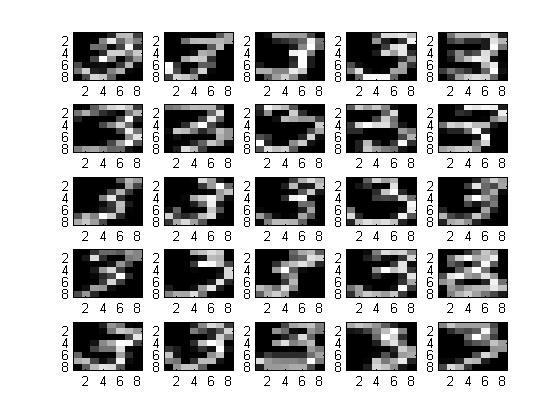
\includegraphics[width=3.2in]{3} 
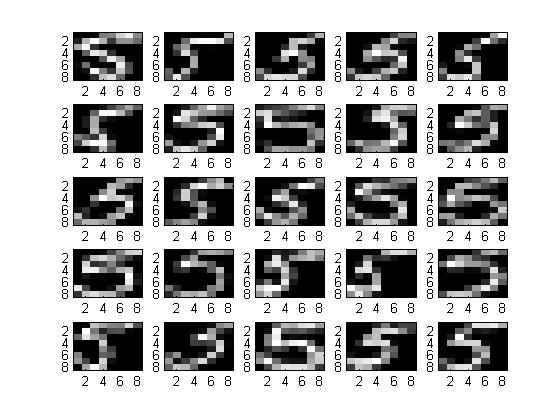
\includegraphics[width=3.2in]{5}\\

\hspace{1in} 1) Data plot for 3    \hspace{2in} 2) Data plot for 5


\cleardoublepage 

\section{Method Classification}

From the question 4 we have derived that:\\

1. p($C_k$) = P(t = k) = $\pi_k$ = $\frac{N_k}{N}$\\

2. p($x|t = k,\mu_k,\Sigma_k$) = $(2\pi)^{-D/2}|\Sigma|^{1/2}$exp$(-\frac{1}{2}(x_n-\mu_k)^T\Sigma^{-1}(x_n-\mu_k))$, \\ where $\mu_k = \frac{1}{N_k}\sum\limits_{n=1}^N t_{nk}x_n$\\

3. The log posterior \\
lnp($t= k|x$) = ln($p(x|t=k,\mu_k,\Sigma_k)\pi_k$)- ln($p(x|t=0,\mu_0,\Sigma_0)\pi_0+p(x|t=1,\mu_1,\Sigma_1)\pi_1$)
\\

4. $\Sigma_k = \frac{1}{N_k} \sum\limits_{n=1}^N t_{nk}(x_n-\mu_k)(x_n-\mu_k)^T$\\

\section{Output analysis}
Table below shows the average conditional probability of Test set and training set\\

\begin{verbatim}
		Average Log Conditional Probability of Training data
________________________________________________________________
        | Conditional Gaussian   Regularized Conditional Gaussian
________|________________________________________________________
Number 3|  -0.135151472698277       -0.049105198331912
Number 5|  -0.276712498340588       -0.053870587663031
Overall |  -0.205931985519433       -0.051487892997471


		Average Log Conditional Probability of Test data
________________________________________________________________
        | Conditional Gaussian   Regularized Conditional Gaussian
________|________________________________________________________ 
Number 3|  -0.032987865886690      -0.006468977130022
Number 5|  -1.262579785698999      -0.212511104167940
Overall |  -0.647783825792844      -0.109490040648981

\end{verbatim}
 \cleardoublepage
  Table below shows the training and testing error for the two different classifier \\

\begin{verbatim}
		Error Counts and Rate of Training Data
________________________________________________________________
        | Conditional Gaussian    Regularized Conditional Gaussian
________|________________________________________________________
        | Error Count Error Rate  Error Count Error Rate  
Number 3|    5.0000    0.0125      3.0000     0.0075
Number 5|    6.0000    0.0100      4.0000     0.0067
Overall |   11.0000    0.0138      7.0000     0.0088


			Error Counts and Rate of Testing Data 
________________________________________________________________
________________________________________________________________
        | Conditional Gaussian    Regularized Conditional Gaussian
________|________________________________________________________
        | Error Count Error Rate  Error Count Error Rate  
Number 3|    2.0000    0.0100            0         0
Number 5|    9.0000    0.0450       6.0000    0.0300
Overall |   11.0000    0.0275       6.0000    0.0150
\end{verbatim}

From the result, it's obvious that regularization hlpes to reduce the overall error rate on both training data and testing data. In addition, we notice that the error rate for Number 3 is smaller than the error rate for Number 5 in both dataset and classifiers. Error rate in Training data is lower than that in Testing data.

\cleardoublepage
\section{Appendic}
\begin{verbatim}
train = textread('digitstrain.txt','','delimiter',',');
test = textread('digitstest.txt','','delimiter',',');
zero = [];
one  = [];
for i = 1:length(train)
if train(i,65) == 0;
    zero = [zero;train(i,:)];    
else
    one = [one;train(i,:)];
end
end

figure;
for i = 1:25
temp = vec2mat(zero(i,1:64),8);
subplot(5,5,i)
imagesc(temp);
colormap(gray);
end

figure;
for i = 1:25
temp = vec2mat(one(i,1:64),8);
subplot(5,5,i)
imagesc(temp);
colormap(gray);
end

%MLE SOLUTION
N = length(train);
N5 = sum(one(:,65));
N3 = N - N5;
pi3 = N3/N;
pi5 = N5/N;
mu3 = sum(zero(:,1:64))/N3;
mu5 = sum(one(:,1:64))/N5;

%Determine the sigma matrix 
S3 = zeros(64);
S5 = zeros(64);
for i=1:N3
    S3 = S3 + transpose(zero(i,1:64)-mu3)*(zero(i,1:64)-mu3);
end
S3 = S3/N3;

for i=1:N5
    S5 = S5 + transpose(one(i,1:64)-mu5)*(one(i,1:64)-mu5);
end
S5 = S5/N5;

%Regularization
S3_r = S3 + 0.01*eye(64) ;
S5_r = S5 + 0.01*eye(64) ;

%main 
train_Cond = zeros(1,N);
train_RCond = zeros(1,N);
test_Cond = zeros(1,length(test));
test_RCond = zeros(1,length(test));

for i = 1:N
    train_Cond(i) = lnp_t(train(i,1:64),train(i,65),S3,S5,mu3,mu5);
    train_RCond(i) = lnp_t(train(i,1:64),train(i,65),S3_r,S5_r,mu3,mu5);
   
end
N_t = length(test);
for i = 1:N_t
    test_Cond(i) = lnp_t(test(i,1:64),test(i,65),S3,S5,mu3,mu5);
    test_RCond(i) = lnp_t(test(i,1:64),test(i,65),S3_r,S5_r,mu3,mu5);
   
end
train_Cond_3 = mean(train_Cond(find(train(:,65)==0)));
train_Cond_5 = mean(train_Cond(find(train(:,65)==1)));
train_RCond_5 = mean(train_RCond(find(train(:,65)==1)));
train_RCond_3 = mean(train_RCond(find(train(:,65)==0)));


test_Cond_3 = mean(test_Cond(find(test(:,65)==0)));
test_Cond_5 = mean(test_Cond(find(test(:,65)==1)));
test_RCond_5 = mean(test_RCond(find(test(:,65)==1)));
test_RCond_3 = mean(test_RCond(find(test(:,65)==0)));


res_train = transpose([train_Cond_3,train_Cond_5,mean(train_Cond);
             train_RCond_3,train_RCond_5,mean(train_RCond)]);
res_test = transpose([test_Cond_3,test_Cond_5,mean(test_Cond);
             test_RCond_3,test_RCond_5,mean(test_RCond)]);

train_Cond_pre =  zeros(1,N);
train_RCond_pre = zeros(1,N);
test_Cond_pre = zeros(1,N_t);
test_RCond_pre = zeros(1,N_t);

for i=1:N
    
    if lnp_x(train(i,1:64),0,S3,S5,mu3,mu5)>
    lnp_x(train(i,1:64),1,S3,S5,mu3,mu5)
            train_Cond_pre(i) = 0;
    else train_Cond_pre(i) = 1;    
    end    
    if lnp_x(train(i,1:64),0,S3_r,S5_r,mu3,mu5)
    >lnp_x(train(i,1:64),1,S3_r,S5_r,mu3,mu5)
            train_RCond_pre(i) = 0;
    else train_RCond_pre(i) = 1;    
    end
end

for i=1:N_t
    
    if lnp_x(test(i,1:64),0,S3,S5,mu3,mu5)> lnp_x(test(i,1:64),1,S3,S5,mu3,mu5)
            test_Cond_pre(i) = 0;
    else test_Cond_pre(i) = 1;    
    end    
    if lnp_x(test(i,1:64),0,S3_r,S5_r,mu3,mu5)>
    lnp_x(test(i,1:64),1,S3_r,S5_r,mu3,mu5)
            test_RCond_pre(i) = 0;
    else test_RCond_pre(i) = 1;    
    end
end

%test error
e_test_3_Cond = abs(test_Cond_pre - transpose(test(:,65)));
e_test_3_Cond = sum(e_test_3_Cond(test(:,65)==0));
e_test_5_Cond = abs(test_Cond_pre - transpose(test(:,65)));
e_test_5_Cond = sum(e_test_5_Cond(test(:,65)==1));
e_test_total_Cond = sum(abs(test_Cond_pre - transpose(test(:,65))));

N_t3 = sum(test(:,65)==0);
N_t5 = N_t- N_t3;

e_test_3_RCond = abs(test_RCond_pre - transpose(test(:,65)));
e_test_3_RCond = sum(e_test_3_RCond(test(:,65)==0));
e_test_5_RCond = abs(test_RCond_pre - transpose(test(:,65)));
e_test_5_RCond = sum(e_test_5_RCond(test(:,65)==1));
e_test_total_RCond = sum(abs(test_RCond_pre - transpose(test(:,65))));

test_error_Cond = [e_test_3_Cond,e_test_3_Cond/N_t3;
              e_test_5_Cond,e_test_5_Cond/N_t5;
              e_test_total_Cond, e_test_total_Cond/N_t;
             ];
test_error_RCond = [e_test_3_RCond,e_test_3_RCond/N_t3;
              e_test_5_RCond,e_test_5_RCond/N_t5;
              e_test_total_RCond, e_test_total_RCond/N_t;
             ];

%training error
e_train_3_Cond = abs(train_Cond_pre - transpose(train(:,65)));
e_train_3_Cond = sum(e_train_3_Cond(train(:,65)==0));
e_train_5_Cond = abs(train_Cond_pre - transpose(train(:,65)));
e_train_5_Cond = sum(e_train_5_Cond(train(:,65)==1));
e_train_total_Cond = sum(abs(train_Cond_pre - transpose(train(:,65))));

N_3 = sum(train(:,65)==0);
N_5 = N- N_t3;

e_train_3_RCond = abs(train_RCond_pre - transpose(train(:,65)));
e_train_3_RCond = sum(e_train_3_RCond(train(:,65)==0));
e_train_5_RCond = abs(train_RCond_pre - transpose(train(:,65)));
e_train_5_RCond = sum(e_train_5_RCond(train(:,65)==1));
e_train_total_RCond = sum(abs(train_RCond_pre - transpose(train(:,65))));

train_error_Cond = [e_train_3_Cond,e_train_3_Cond/N_3;
              e_train_5_Cond,e_train_5_Cond/N_5;
              e_train_total_Cond, e_train_total_Cond/N;
             ];
train_error_RCond = [e_train_3_RCond,e_train_3_RCond/N_3;
              e_train_5_RCond,e_train_5_RCond/N_5;
              e_train_total_RCond, e_train_total_RCond/N;
             ];
% % % % % % % % % % % % % % % % % % % % % % % %
function [res] = lnp_t(x,t,S0,S1,mu0,mu1)
res = lnp_x(x,t,S0,S1,mu0,mu1) -log(exp(lnp_x(x,0,S0,S1,mu0,mu1))+exp(lnp_x(x,1,S0,S1,mu0,mu1)));
end
% % % % % % % % % % % % % % % % % % % % % % % % 

% % % % % % % % % % % % % % % % % % % % % % % %
function [res] = lnp_x(x,t,S0,S1,mu0,mu1)
D = 64;
if t == 0;
    res  = -D/2 * log(2*pi) - log(det(S0))/2 - ((x-mu0)*inv(S0)*transpose(x-mu0))/2;
else    
    res = -D/2 * log(2*pi) - log(det(S1))/2 - ((x-mu1)*inv(S1)*transpose(x-mu1))/2;
end
end
% % % % % % % % % % % % % % % % % % % % % % % % 



\end{verbatim}
\end{document}